\section{Architecture}
\label{sec:architecture}
\begin{figure*}[!t]
  \centering
  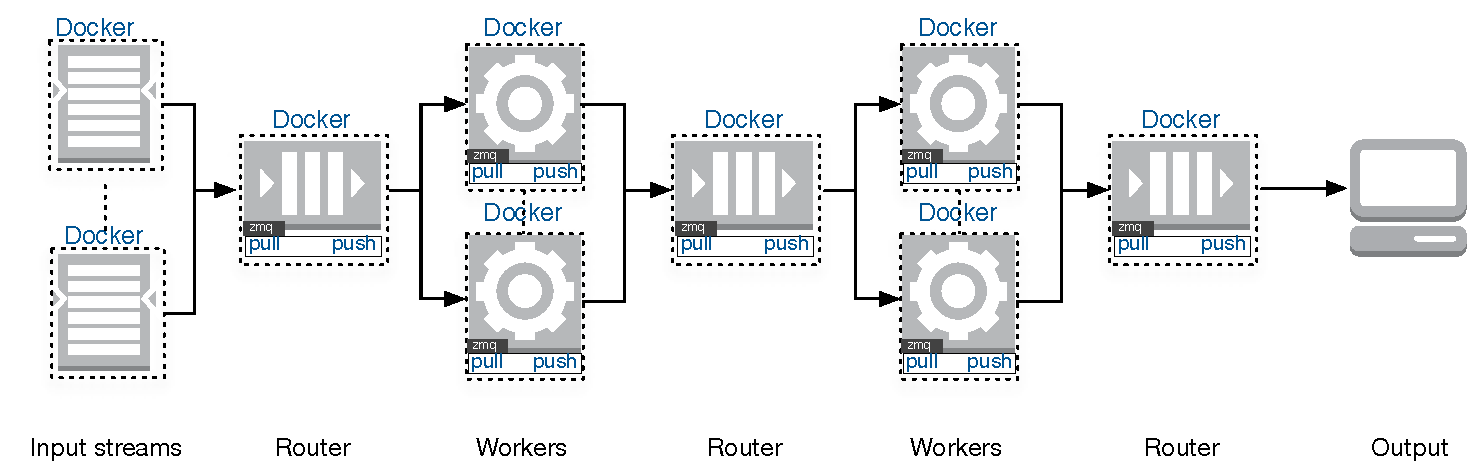
\includegraphics[scale=0.7]{images/architecture_pipeline}
  \caption{Example of \SYS pipeline architecture.\vs{I will tune a bit the image}}
  \label{fig:architecture_pipeline}
\end{figure*}

% \begin{itemize}
%   \item Communication by ØMQ (version 4.1.4)
%   \item Docker container for clustered deployment
%   \item Workers connected by routers: define worker's role and router's operating
%   \item Fire-and-forget messaging: a messsaging pattern in which we do not expect a direct response to the message, as opposed to request-response protocols
%   \item Based on Lua
% \end{itemize}

The architecture of \textsc{SecureStreams} comprises of a combination two different types of components: worker and routers.
A worker component executes continuously listen for incoming data by means of non-blocking I/O.
As soon as a data flows in, some application-dependent business logic is applied.
A typical use-case is the deployment of a MapReduce processing pipeline~\cite{Dean:2008:MSD:1327452.1327492}, with worker nodes that execute \texttt{map}, \texttt{filter} and \texttt{reduce} functions.
Router act as message brokers between workers in the pipeline and transfer data between workers according to some dispatching policy.
Figure~\ref{fig:architecture_pipeline} depicts a possible implementation of MapReduce using the \SYS middleware.
%Datas in \textsc{SecureStreams} are streamed accross the process pipeline as shown in figure \ref{fig:architecture_pipeline}.

\textsc{SecureStreams} is designed to allow processing of sensible data inside SGX enclaves.
However, the Enclave Page Cache (EPC) is currently limited at 128 MB.
To overcome these limitations, we settled on a lightweight yet efficient embeddable runtime based on the Lua Virtual Machine\cite{ierusalimschy_luaextensible_1996} and the corresponding multi-paradigm scripting language~\cite{lualang}.
Note that the Lua runtime requires only few kB of memory, and thus representing an ideal candidate to execute in the limited space allowed by the EPC.
The application-specific functions can be quickly prototyped in Lua.
%If a process exceeds the available memory, an encrypted pagination mechanism leads to performance leaks.
%Thus \textsc{SecureStreams} has been designed to use a Lua runtime.
%Lua is a lightweight multi-paradigm programming language designed primarily for embedded systems and clients\cite{ierusalimschy_luaextensible_1996}.
%Its runtime requires only few KB of memory, and thus fits easily in EPC.
Each component is wrapped inside a Docker container to easily embed all required dependencies and ensure the correctness of their configuration.
By doing so, a processing pipeline can be easily deployed on different infrastructures, such as the Amazon EC2 Container Service~\cite{awsec2container}, either on a single machine or a cluster, using a Docker network and the Docker Swarm\cite{docker:swarm_2016} scheduler.

The communication between workers and routers leverages \zmq, a high-performance asynchronous messaging library~\cite{zero_mq}.
Each router component hosts inbound and outbound queues. %\vs{how much?}\ah{We don't know, so we should not talk about queue size. BTW, I don't understand your sentence. Do you missed a verb?}.
In particular, we use the \zmq's pipeline pattern with the \emph{PUSH}-\emph{PULL} protocol\cite{zero_mq:pipeline}.
The inbound queue is a \emph{PULL} socket.
The messages are streamed from a set of anonymous\footnote{Anonymous is said about a peer without any identity, the server socket does not know which worker sent the message} \emph{PUSH} peers (e.g. the upstream workers in the pipeline).
The inbound queue uses a fair-queuing scheduling to deliver the message to the upper layer.% dispatches the messages.\ah{that's not true, the fair-queuing algorithm operates at the level of the reception of the queue, and it does not dispatch anything, the message is passed to the outgoing socket/queue, that's it}
Conversely, the outbound queue is a \emph{PUSH} socket, sending messages using a round-robin algorithm to a set of anonymous \emph{PULL} peers, the downstream workers.
\vs{if there is time, it could be useful to have a drawing that zooms into this aspect of the architecture, not the full pipeline}
This design allows to dynamically scale up/down each stage of the pipeline. %It is scalable in that nodes can join at any time.
Finally, \zmq guarantees that the messages are delivered across each stage via reliable TCP channels.
%The pattern is mostly reliable insofar as it will not discard messages unless a node disconnects unexpectedly.
%This fire-and-forget messaging is a messsaging pattern in which we do not expect a direct response to the message, as opposed to request-response protocols\cite{voelter_patterns_2003}.
% The absence of response to a message provides some relevant performances.


